\subsection{1D pulse--acquire}
\label{subsec:theory__pulseacq}

Consider the simplest NMR experiment, a 1D \proton{} pulse--acquire spectrum (\cref{fig:pulse_acquire}).
This consists of a \ang{90} pulse, immediately followed by detection; for convenience, we will first consider the pulse as being applied along the $+y$-axis, i.e. with a phase of $\phi = \pi/2$.

\begin{figure}[htbp]
    \centering
    \label{fig:pulse_acquire}
    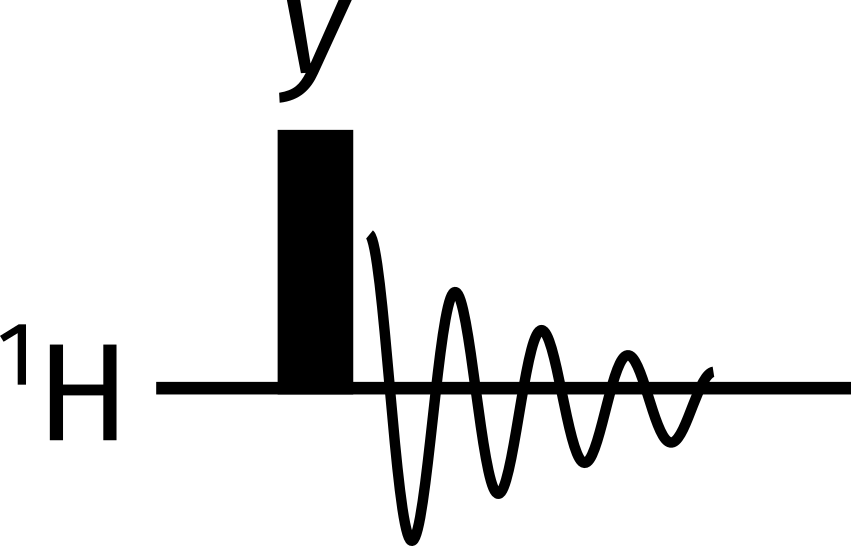
\includegraphics[]{pp/zg_y.png}
    \caption[Pulse--acquire experiment]{1D \proton{} pulse--acquire experiment.}
\end{figure}

To understand this, we begin with the thermal density operator $\rho_0' = I_z$ (\cref{eq:rho0_simplified}) and assume that there is only one spin in the sample, and that the pulse is applied on-resonance.
The corresponding Hamiltonian during the pulse is simply $\omega_1 I_y$ (\cref{eq:hard_pulse_onresonance}).
If the duration of the pulse is $\taup$, then the density operator immediately following the pulse is given by:
\begin{equation}
    \label{eq:rho_after_pulse}
    \rho = \exp(-\mi\omega_1 I_y\taup) I_z \exp(\mi\omega_1 I_y\taup) = \cos(\omega_1\taup)I_z + \sin(\omega_1\taup)I_x.
\end{equation}
In this case, to obtain a \ang{90} pulse, $\taup$ is specifically calibrated to ensure that $\omega_1\taup = \pi/2$, which yields
\begin{equation}
    \label{eq:rho_after_pulse_simplified}
    \rho = I_x.
\end{equation}
During the detection period, this term evolves under $H_\text{free} = H_\text{cs} = \omega_0 I_z$.
(We use the Schr\"odinger-picture free Hamiltonian here because the measurement of the NMR signal takes place in the laboratory frame.)
At a time $t$ after detection has begun, the density operator is thus:
\begin{equation}
    \label{eq:rho_during_detection}
    \rho(t) = \exp(-\mi \omega_0 I_z t)I_x\exp(\mi\omega_0 I_z t) = \cos(\omega_0 t)I_x + \sin(\omega_0 t)I_y.
\end{equation}
The NMR signal derives from both $x$- and $y$-magnetisation ($M_x$ and $M_y$), which are in turn proportional to $I_x$ and $I_y$ by a factor of $\gamma$.
(If multiple spins are present, then each spin induces its own magnetisation: we would have that $M_x = \sum_i \gamma_i I_{ix}$, and likewise for $M_y$.)
These are then combined to form a complex signal (this process is known as \textit{quadrature detection}):
\begin{align}
    s(t) &= M_x(t) + \mi M_y(t) \label{eq:quadrature} \\
         &\propto \langle I_x(t) \rangle + \mi \langle I_y(t) \rangle \notag \\
         &= \Tr[I_x\rho(t)] + \mi \Tr[I_y\rho(t)] \notag \\
         &\propto \cos(\omega_0 t) + \mi \sin(\omega_0 t) \notag \\
         &= \exp(\mi \omega_0 t). \label{eq:fid}
\end{align}
Before the signal is digitised, the NMR spectrometer mixes this with a \textit{reference} RF field oscillating at the transmitter frequency $\omega_\text{tx}$.
This results in downconversion of the detected frequencies by $\omega_\text{tx}$, such that the actual digitised signal oscillates at the offset frequency $\Omega$ rather than $\omega_0$ (recall we have chosen $\omega_\text{rot} = \omega_\text{tx}$, so $\omega_0 - \omega_\text{tx} = \omega_0 - \omega_\text{rot} = \Omega$).
Therefore, instead of \cref{eq:fid}, the signal we really see is:
\begin{equation}
    \label{eq:fid_reduced}
    s(t) \propto \exp(\mi \Omega t).
\end{equation}
This result is the same as if we had pretended that during the detection period, $\rho$ evolved under the \textit{interaction-picture} free Hamiltonian $H_{\text{free},I} = H_\text{offset}$; we will henceforth adopt this simplification, even though it is not physically accurate.

In practice, relaxation causes this signal to decay with time; this is frequently modelled as an exponential, in accordance with the Bloch equations\autocite{Bloch1946PR}:
\begin{equation}
    \label{eq:fid_with_relaxation}
    s(t) = \exp(\mi\Omega t)\exp(-t/T_2),
\end{equation}
where $T_2$ is the transverse relaxation time.\footnote{Transverse (and longitudinal) relaxation are sometimes called spin--spin (and spin--lattice) relaxation, although the continued usage of these terms has been criticised\autocite{Levitt2008,Keeler2010,Gupta2021JPCL}.}
The NMR signal is thus often called a \textit{free induction decay} (FID).
Fourier transformation of the FID then yields a spectrum with absorption- and dispersion-mode lineshapes in the real and imaginary parts respectively (\cref{fig:lorentzians}):
\begin{equation}
    \label{eq:lorentzian}
    S(\omega) = \mathcal{F}[s(t)] =
    \underbrace{\frac{k}{k^2 + (\omega - \Omega)^2}}_{A(\omega; \Omega)}
    +\, \mathrm{i}\underbrace{\frac{\Omega - \omega}{k^2 + (\omega - \Omega)^2}}_{D(\omega; \Omega)},
\end{equation}
where $k = 1/T_2$.
The notation $A(\omega; \Omega)$ here means that the spectrum is a function of the frequency $\omega$, but is parametrised by the peak offset $\Omega$.
Conventionally, only the real part of the spectrum is displayed, so it is desirable for the real part to contain the absorption-mode lineshape.
This provides better resolution due to the narrower lineshape, and is also less affected by cancellation when multiple peaks overlap.

\begin{figure}[htbp]
    \centering
    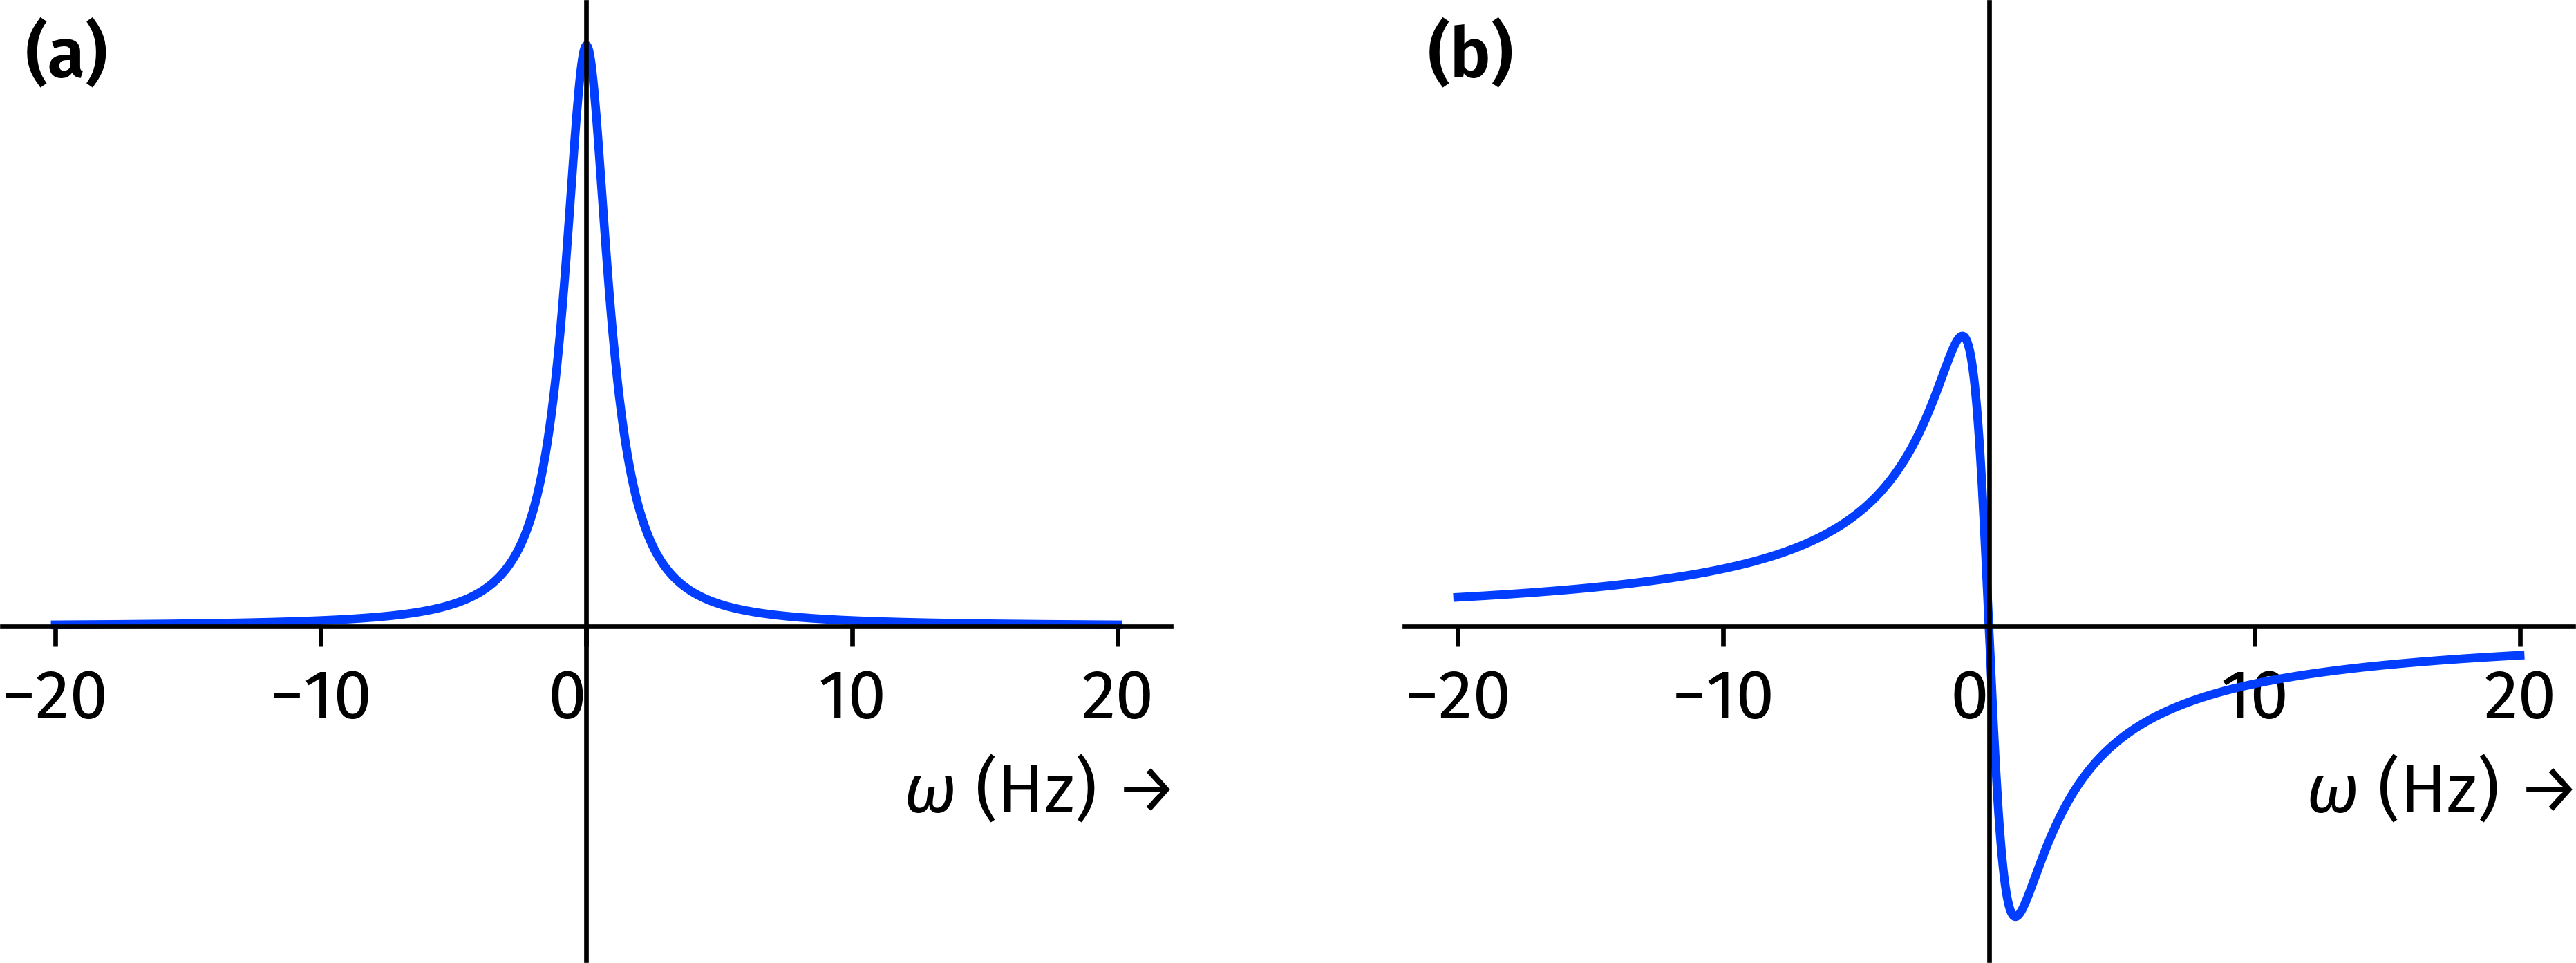
\includegraphics[]{theory/lorentzians.png}
    {\phantomsubcaption\label{fig:lorentzians_absorption}}
    {\phantomsubcaption\label{fig:lorentzians_dispersion}}
    \caption[Absorption- and dispersion-mode Lorentzian lineshapes]{
        \textbf{(\subref{fig:lorentzians_absorption})} Absorption-mode lineshape $A(\omega; \Omega = 0)$.
        \textbf{(\subref{fig:lorentzians_dispersion})} Dispersion-mode lineshape $D(\omega; \Omega = 0)$.
        Both lines have been plotted using $k = \SI{\pi}{\radian\per\second}$.
    }
    \label{fig:lorentzians}
\end{figure}

Strictly speaking, the Lorentzian lineshapes above are only obtained when there is nonzero relaxation during the FID.
For example, in the limit $k \to 0$, $A(\omega; \Omega)$ tends to a delta function $\delta(\omega = \Omega)$.
However, for simplicity, in this thesis I will drop the relaxation term $\exp(-kt)$ unless absolutely necessary; I will simply pretend that a signal of the form $s(t) = \exp(\mi \Omega t)$ is directly Fourier transformed to give $A(\omega; \Omega) + \mi D(\omega; \Omega)$.

Consider now changing the initial pulse such that it is applied along the $+x$-axis instead ($\phi = 0$).
Repeating the above analysis, we find that the resulting signal will have a phase shift:
\begin{align}
    \label{eq:fid_phase_shifted}
    s'(t) &= -\mi\exp(\mi\Omega t) \\
    \Rightarrow \quad S'(\omega) &= \mathcal{F}[s'(t)] = D(\omega;\Omega) - \mi A(\omega;\Omega).
\end{align}
If we were to take the real part of the spectrum here, then we would obtain the undesired dispersion-mode lineshape $D(\omega;\Omega)$.
There are two ways of removing this phase shift.
The first is to shift the \textit{receiver phase} by $\phi_\text{rec}$, which introduces an extra factor of $\exp(-\mi\phi_\text{rec})$ to the detected signal: we can thus choose $\phi_\text{rec} = 3\pi/2$ in order to cancel out the $-\mi$ term in $s'(t)$.
Alternatively, the spectrum can be processed through \textit{phase correction}, in which $S(\omega)$ is directly multiplied by a term $\exp(\mi\phi_\text{corr})$, where $\phi_\text{corr}$ is a linear function of the frequency $\omega$:
\begin{equation}
    \label{eq:phase_correction}
    \phi_\text{corr} = \phi_{\text{corr}}^{(0)} + \omega\phi_{\text{corr}}^{(1)}.
\end{equation}
$\phi_\text{corr}^{(0)}$ and $\phi_\text{corr}^{(1)}$ are respectively termed the \textit{zeroth-} and \textit{first-order phase corrections}: in this idealised case, we can simply choose $(\phi_\text{corr}^{(0)}, \phi_\text{corr}^{(1)}) = (\pi/2, 0)$ to again remove the unwanted phase shift.
More realistically, due to instrumental imperfections, both of these values will have to be nonzero in order to ensure that every peak in the spectrum has the correct phase, i.e.\ is displayed in absorption-mode.

An alternative framework for analysing pulse sequences is to use the ladder operators $I_+$ and $I_-$ (\cref{eq:other_single_spin_ops}).
Using the original example with our initial pulse on $+y$, the density operator immediately after the pulse is:
\begin{equation}
    \label{eq:rho_coherences}
    \rho = I_x = \frac{1}{2}(I_+ + I_-),
\end{equation}
and during detection this evolves as:
\begin{equation}
    \label{eq:fid_coherences}
    \rho(t) = \cos(\Omega t)I_x + \sin(\Omega t)I_y = \frac{1}{2}\left[\exp(-\mi \Omega t)I_+ + \exp(\mi \Omega t)I_- \right].
\end{equation}
(Notice that the $+1$-coherence $I_+$ actually evolves at the negative frequency $-\Omega$.)
To obtain the same signal as previously done in \cref{eq:fid}, we `detect' the $I_-$ term:
\begin{equation}
    \label{eq:detection_coherences}
    s(t) \propto \Tr[I_- \rho(t)] \propto \exp(\mi\Omega t),
\end{equation}
which leads to the common assertion that \textit{only quantum coherences of order $-1$ are detectable}.
It is true that coherences with orders $p = 0, \pm 2, \pm 3, \ldots$ can never be detected in an FID.
However, it is worth pointing out that the `uniqueness' of $-1$-coherence is merely a result of how the $x$- and $y$-magnetisation are combined to form the complex signal (\cref{eq:quadrature}).
We do not \textit{physically} detect $I_-$: we detect $I_x$ and $I_y$, and combine them to form a complex signal which is mathematically equal to detecting $I_-$.
If we had instead chosen to combine them in a different way, such as $s(t) = M_x(t) - \mi M_y(t)$, this would give us $s(t) \propto \exp(-\mi\Omega t)$---corresponding to `detection' of $+1$-coherence---although this alternative does come with the drawback that frequencies must be reversed after Fourier transformation.
In any case, we will stick to the established convention of detecting $-1$-coherence here.

To end this section, it should be pointed out that the complex signal is not obtained as an infinitely-long, continuous function of time, as the treatment above implies.
The complex-valued signal is digitised at an interval called the \textit{dwell time}, $\tau_\text{dw}$, and detection must be stopped after a finite period called the \textit{acquisition time}, $\tau_\text{aq}$.
The FT being performed is actually a discrete Fourier transform (DFT), which yields a periodic function $S(\omega)$; its period (in Hz) is given by $1/\tau_\text{dw}$.%
\footnote{The periodicity property of the DFT is equivalent to the Nyquist theorem, which is usually formulated as follows: the sampling rate required to correctly digitise a signal containing frequencies in the range $[0, f_\text{max}]$ is $1/(2f_\text{max})$. In the main text, it appears as if we have dropped the factor of $2$ in the denominator; but in truth this statement of the Nyquist theorem is applicable to \textit{real-valued} signals, and here we have a \textit{complex-valued} signal $s(t)$, which effectively doubles the range of correctly sampled frequencies.}
The NMR spectrum displayed to the user corresponds to one single period of $S(\omega)$, and thus the \textit{spectral width} is also equal to $1/\tau_\text{dw}$.%
\footnote{Frustratingly, the \texttt{DW} parameter in Bruker's TopSpin software is actually equal to $\tau_\text{dw}/2$. The reason is because this parameter corresponds to the interval between which \textit{real} data is sampled, which is effectively twice as fast as complex-valued sampling.}
In principle, the periodicity of the DFT means that signals which would ordinarily fall outside of the spectral width would appear at incorrect frequencies in the spectrum.\autocite{Turner1986JMR}
On modern instrumentation, this is no longer the case for direct detection; peaks outside of the spectral width are removed using digital filters.
However, \textit{folding} or \textit{aliasing} of peaks in the indirect dimension(s) of multidimensional NMR spectra still occurs.

The DFT $S(\omega)$ is also a discrete function itself, and its resolution is given by $1/\tau_\text{aq}$.
It is possible to extend the effective acquisition time (and thus improve spectral resolution) without actually acquiring more data: this can be done either by \textit{forward linear prediction} of the signal, or by simply adding zeros onto the end of the signal (\textit{zero-filling}).
